\chapter{Current Work}
\label{currentwork}

The aim of this research is to construct a process calculus which
combines the notions of discrete time and mobility.  Earlier work
during an undergraduate project focused on developing a semantics for
the Cashews\footnote{Cashews is a language for web service
  composition, initially based on OWL-S.}\cite{cashews-sem} language,
using the CaSE process calculus (see section \ref{tplext}) and later,
a conservative extension to it called Cashew-Nuts.  It became clear
during this project that it would be interesting to further extend CaSE
with a notion of mobility, and this lead to the development of the
calculus of \emph{Typed Nomadic Time} (TNT) discussed here.

\section{The Calculus of Synchronous \\ Encapsulation (CaSE)}
\label{case}

The syntax for CaSE, given in \cite{norton05alg}, is as follows:

\begin{equation}
  \begin{aligned}
    \expr, \exprb\ ::=\ &
    \nil  \;\,|\,\; 
    \Delta \;\,|\,\; 
    \Delta_{\sigma} \;\,|\,\; 
    \alpha . \expr  \;\,|\,\;
    \expr + \exprb \;\,|\,\; 
    (\expr\;|\;\exprb)\;\,|\,\; 
    \timeout{\expr}{\sigma}{\exprb} \;\,|\,\; \\
    & \stimeout{\expr}{\sigma}{\exprb} \;\,|\,\; 
    \mu X . \expr \;\,|\,\; 
    X \;\,|\,\; 
    \expr \setminus a \;\,|\,\; 
    \expr / \sigma
  \end{aligned}
\end{equation}

\noindent where $\alpha$ is as in the definition of CCS (see \ref{ccs}).
$\nil$, $\alpha.\expr$, $\expr + \exprb$, $(\expr\;|\;\exprb)$, $\mu X
. \expr$, $X$ and $\expr \setminus a$ retain their behaviour defined in
CCS, but now exhibit additional actions due to the presence of clocks.
These are drawn from a countably infinite set, $\timers$, over which
$\sigma$ ranges.

There are now transitions for the $\nil$ process, as, while the
process has no explicit behaviour, it can idle over the ticks of the
clocks.  This also applies to actions in general:

\begin{equation}
a.0 \derives{\sigma} a.0
\end{equation}

\noindent assuming a clock context containing just the one clock,
$\sigma$. Similarly, non-deterministic choice and parallel composition
exist through time, so either side can evolve due to a clock tick,
while the operator remains in place.  This gives the following
possible derivations for $a.0\;|\;b.0$ (where $b \ne \overline{a}$):

\begin{enumerate}
\item $a.0\ |\ b.0 \derives{a} 0\ |\ b.0$
\item $a.0\ |\ b.0 \derives{b} a.0\ |\ 0$
\item $a.0 |\ b.0 \derives{\sigma} a.0\ |\ b.0$
\end{enumerate}

\noindent with the same clock context as above.  The third derivation
is duplicated for each available clock that can tick over both sides
of the composition.  In cases where both sides may synchronize,
causing a $\tau$ transition, this takes precedence over the clock
transitions, due to \emph{maximal progress} (see \ref{timing}) and the
original set of derivations for parallel composition (see \ref{ccs})
are available instead.

The changes to non-deterministic choice are simpler, as the operator itself
does not generate silent actions.  So, if both sides allow the clock to tick,
then the following derivations will occur:

\begin{enumerate}
\item $a.0\ +\ b.0 \derives{a} 0$
\item $a.0\ +\ b.0 \derives{b} 0$
\item $a.0\ +\ b.0 \derives{\sigma} a.0\ +\ b.0$
\end{enumerate}

\noindent again with the single clock, $\sigma$, as the context.

\subsection{Timeouts}

Moving on to the new operators, CaSE, as presented in
\cite{norton05alg}, includes two variants of the timeout operator,
first seen in TPL.  Recall from \ref{timing} that the operator
essentially allows a decision to be made, based on the presence of a
clock tick.  In the general scenario,

\begin{equation}
\timeout{E}{\sigma}{F}
\end{equation}

\noindent $F$ will act if $E$ fails to, prior to a clock tick.  If $E$
can perform a $\tau$ action, then this will prevent the clock tick and
$E$ will evolve. Both operators in CaSE maintain this core behaviour,
which is central to the concept of global synchronization explained
earlier.

The difference between the two operators in CaSE lies in their
behaviour with regard to other clocks.  With the fragile timeout,
$\timeout{E}{\sigma}{F}$, any possible transition on $E$ will cause the
removal of the timeout.  So, with $\timeout{a.0}{\sigma}{b.0}$ and a clock
context of $\sigma$ and $\rho$, the following derivations can occur:

\begin{enumerate}
\item $\timeout{a.0}{\sigma}{b.0} \derives{a} 0$
\item $\timeout{a.0}{\sigma}{b.0} \derives{\sigma} b.0$
\item $\timeout{a.0}{\sigma}{b.0} \derives{\rho} a.0$
\end{enumerate}

\noindent where both the $a$ and the $\rho$ transition leave only the
left-hand side of the timeout.

The stable timeout differs by continuing to exist through time until
some action occurs.  While it exhibits the same behaviour in response
to actions or the tick of the specified clock, the ticks of other
clocks only cause the left-hand side to evolve; the timeout itself is
retained.  Thus, $\stimeout{a.0}{\sigma}{b.0}$ gives a different set
of derivations:

\begin{enumerate}
\item $\stimeout{a.0}{\sigma}{b.0} \derives{a} 0$
\item $\stimeout{a.0}{\sigma}{b.0} \derives{\sigma} b.0$
\item $\stimeout{a.0}{\sigma}{b.0} \derives{\rho} \stimeout{a.0}{\sigma}{b.0}$
\end{enumerate}

\noindent where the $\rho$ transition no longer causes the dissolution
of the timeout.

\subsection{Clock Stopping and Insistency}
\label{clockcontrol}

The remaining operators further control the behaviour of the clocks.
$\Delta$ prevents all clocks from ticking, while $\Delta_{\sigma}$
prevents only the ticks of the specified clock, $\sigma$.  $\Delta$ is
similar to the CCS version of $\nil$, as it has no possible
transitions.  $\Delta_{\sigma}$ exhibits transitions for all other
clocks within the current context.  So, for a context containing both
$\sigma$ and $\rho$, $\Delta_{\sigma}$ has a single transition,

\begin{equation}
  \Delta_{\sigma} \derives{\rho} \Delta_{\sigma}
\end{equation}

\noindent which is replicated for any other clocks in the context,
which are not equal to $\sigma$.

The stopping of clocks is used to provide \emph{insistency}.  Normally,
a process $a.P$ has two possible derivations:

\begin{enumerate}
  \item $a.P \derives{a} P$
  \item $a.P \derives{\sigma} P$
\end{enumerate}

\noindent with a clock context containing only $\sigma$.  To ensure
that the first of these two derivations occurs, or, in other words, to
\emph{insist} that $a$ is performed before the next tick of the clock,
$\sigma$, $\Delta$ is used.  The semantics for an insistent prefix,
$\underline{\alpha}.P$, may be given as:

\begin{equation}
\seml \underline{\alpha}.P \semr \eqdef \alpha.P + \Delta 
\end{equation}

\noindent where the presence of $\Delta$ prevents a $\sigma$
transition from occuring on the right-hand side of the choice, and
thus for the choice as a whole (as both sides must move through time
simultaneously).  This leaves only one available action,
$\derives{a}$, as required.  Clearly, insistency relative only to one
particular clock may also be defined in a similar manner, using
$\Delta_{\sigma}$ instead.

\begin{equation}
\seml \underline{\alpha}_{\sigma}.P \semr \eqdef \alpha.P + \Delta_{\sigma} 
\end{equation}

While on the subject of derived syntax, it is also possible to define
a clock prefix, akin to the existing action prefix:

\begin{equation}
\seml \sigma.P \semr \eqdef \stimeout{\nil}{\sigma}{P}
\end{equation}

\noindent where the stable timeout ensures that the $\sigma.P$ will be
retained until $\sigma$ ticks, despite the ticks of other clocks.  As
the only transitions for $\nil$ are clock ticks, only a tick from
$\sigma$ will cause the process to evolve and become $P$.

The two notions of a clock prefix and insistency can then be combined
to give an insistent clock prefix:

\begin{equation}
\seml \underline{\sigma}.P \semr \eqdef \stimeout{\Delta}{\sigma}{P}
\end{equation}

\noindent which differs from a standard clock prefix by only ever
allowing the one transition, $\underline{\sigma}.P \derives{\sigma}
P$, whereas $\sigma.P$ allows an arbitrary number of transitions from
other clocks before this occurs.

\subsection{Encapsulation}

Clock hiding is used to providing scoping for the ticks of a
clock.  Take the following situation,

\begin{equation}
\label{clockhidingex}
  ((P) / \sigma)\;|\;Q
\end{equation}

\noindent where $/ \sigma$ hides the clock, $\sigma$, so that its
ticks may only be seen by $P$.  $Q$ instead sees a silent action each
time $\sigma$ ticks.  Such clock hiding is central to the
encapsulation of components present in CaSE.  When coupled with
restriction, components can be made to only emit silent actions from
the perspective of external processes.

\section{Localising the Calculus}

\emph{Localisation}, discussed in detail in \ref{migration}, effectively
adds another level of grouping to the calculus.  A set of composed
processes may be contained within one \emph{locality}, a notion which is
often used in the modelling of \emph{distribution}.  This idea, which
can be taken to its logical extent by forming a hierarchy of such
localities, has echos of the notion of \emph{clock hiding} within CaSE,
as just described.

Thus, the first step in the evolution towards TNT is to combine these
two hierarchical concepts by effectively localising CaSE.  The notion of
components and encapsulation is explicitly realised by a locality, which
also handles the hiding of clocks.  As a result, the clock hiding
operator from CaSE disappears, being replaced by a new operator which
allows the creation of localities.  The bounds of the locality define
both a new group and the scope of the clock hiding.  The syntax for
localised CaSE is thus:

\begin{equation}
  \begin{aligned}
    \expr, \exprb\ ::=\ &
    \nil  \;\,|\,\; 
    \Delta \;\,|\,\; 
    \Delta_{\sigma} \;\,|\,\; 
    \alpha . \expr  \;\,|\,\;
    \expr + \exprb \;\,|\,\; 
    (\expr\;|\;\exprb)\;\,|\,\; 
    \timeout{\expr}{\sigma}{\exprb} \;\,|\,\; \\
    & \stimeout{\expr}{\sigma}{\exprb} \;\,|\,\; 
    \mu X . \expr \;\,|\,\; 
    X \;\,|\,\; 
    \expr \setminus a \;\,|\,\; 
    \lcloc{m}{\expr}{\vec{\sigma}}
  \end{aligned}
\end{equation}

\noindent where $m$ represents an arbitrary locality name\footnote{Note
that although names are added to the localities here, this is not really
necessary at this stage; they provide nothing more than a way to refer
to localities in talking about a system.  However, they are necessary
for providing migration as discussed in \ref{migration}}; the names of
localities are not distinct, and hence do not form a set.  In
particular, $m$ may be equal to the empty string, $\epsilon$, thus
facilitating the use of anonymous localities.  This allows the semantics
of CaSE's clock hiding to be encoded:

\begin{equation}
\seml E / \sigma \semr \eqdef \lcloc{}{E}{\sigma}
\end{equation}

\noindent thus making localised CaSE a conservative extension.  The
localities form a forest structure, due to the ability to nest
localities to an arbitrary depth and the possibility of multiple
localities occurring at the top level.

Recall the example of clock hiding above (\ref{clockhidingex}).  This
becomes:

\begin{equation}
  \lcloc{}{E}{\sigma}\;|\;Q
\end{equation}

\noindent in localised CaSE, or:

\begin{equation}
  \lcloc{m}{E}{\sigma}\;|\;Q
\end{equation}

\noindent if an arbitrary name, $m$, is assigned to the locality.  Just
as with the clock hiding operator, the clock $\sigma$ is hidden outside
the locality, $m$, causing its ticks to only be visible to $P$.  

With this extension,the set of visible clocks for a particular locality
may be obtained by taking the union of its set of clocks and the sets of
the parent localities.  For example, consider the more complex scenario:

\begin{equation}
\lcloc{n}{E\;|\;\lcloc{m}{F\;|\;\lcloc{k}{G}{\sigma}}{\rho}}{\gamma}
\end{equation}

\noindent where the top-level locality, $n$, contains a process $E$ and
a further sub-locality, $m$.  Likewise, $m$ contains both a process,
$F$, and the sub-locality, $k$.  Finally, $k$ contains just the single
process, $G$.  The set of clocks for the locality $k$ is $\{\sigma\}$
and its parents are $m$ (with the set $\{\rho\}$) and $n$ (with
$\{\gamma\}$).  Thus, the set of visible clocks for $k$ is $\{\sigma\}
\cup \{\rho\} \cup \{\gamma\}$ or simply $\{\sigma, \rho, \gamma\}$,
which means that $G$, located in $k$, can see the ticks of all three
clocks.

$F$, by comparison, can only see the ticks of the clocks, $\rho$ and
$\gamma$, as $\sigma$ is hidden outside $k$.  $E$, in the top-level
locality, $n$, can only observe silent actions resulting from the two
hidden clocks, $\rho$ and $\sigma$, but can see the ticks of $\gamma$.
Taking this further, it is clear that the clock context, the set of
clocks within the system, can be derived as the union of the sets of
clocks associated with each locality ($\{\sigma, \rho, \gamma\}$ in
this case).

\section{Adding Mobility}
\label{addingmob}

Localised CaSE makes the notion of components and encapsulation clearer
than in the original calculus, by allowing them to be given explicit
names.  However, it doesn't provide a great deal of extra
functionality\footnote{Although the semantics could be adapted, so as to
use the localities for bisimulation, as in \ref{migration}}.  The most
natural progression from this stage is to add mobility.  For this, the
primitives of the ambient calculus are adopted, as they provide a very
natural and simplistic formalism, which builds on the component-oriented
nature of the calculus, now explictly realised by localities.  This is
shown in more detail in \ref{locmob}.

In addition, TNT allows the movement of individual processes.  In the
ambient calculus, only ambients can move, which restricts the
separability of processes.  For a given group of processes, the
size of the group may only change by:

\begin{enumerate}
\item One of the processes becoming $\nil$.  The ambient calculus
      includes a structural congruence law,
\begin{equation}
E\;|\;\nil \equiv E
\end{equation}
      which allows such processes to be removed.  Note that this doesn't
      hold for TNT, due to the addition of clocks.  $\nil$ exists
      through time, and, as such, has transitions for each clock.  Thus,
      if $\nil$ is removed from the above equation, there will be fewer
      possible transitions and so it follows that the two should be
      regarded as different processes.
\item The process splitting into two or more processes via parallel
      composition.  For example, $in m.(E | F)$ enters the ambient, $m$,
      and then splits into two separate processes, $E$ and $F$.
\item Another process \emph{open}ing the ambient, causing the set of
      processes to merge with those in the parent.
\end{enumerate}

What the ambient calculus doesn't allow is for a selected process or
group of processes to be moved from one ambient to another.  That
process or group must be in its own ambient for this to happen.

Take the example process, 

\begin{equation}
m[E\;|\;F\;|\;G]\;|\;n[\nil]\;|\;H
\end{equation}

\noindent where $E$, $F$, $G$ and $H$ are all processes and $m$ and $n$
are ambients.  The topology of this may change in several ways, as
outlined above. Any of the four processes may evolve to $\nil$, or fork
into two or more processes.  In addition, $E$, $F$ or $G$ may emit an
$\ambin{n}$ capability, causing the ambient $m$ to move inside $n$.
Similarly, $H$ may perform an $\ambopen{m}$, causing $m$ to be removed and
the top-level to include all four processes.

So, several events may occur but there are also some that are intuitive,
but difficult to achieve.  For instance, all three processes in $m$ must
move as a unit, whether this is to the top-level due to an $open$
capability or as a result of $m$ moving in to $n$.  Moving one process,
$E$ for example, requires the interaction of both $E$ itself and another
process at the final destination.

To move $E$ to the top level on its own requires converting it to the
form,

\begin{equation}
Emov \eqdef z[\ambout{m}.E]
\end{equation}

\noindent where $z$ is a new name, which doesn't occur free in either
$E$, $F$, $G$ or $H$.  The effect is clearer when this is placed in
context,

\begin{equation}
m[z[\ambout{m}.E]\;|\;F\;|\;G]\;|\;n[\nil]\;|\;H
\end{equation}

\noindent where it can be clearly seen that the new capability prefixed
on $E$ will cause the new surrounding ambient, $z$, to move outside of
$m$.  To actually have $E$ at the top-level, and not $E$ nested in an
ambient, requires the presence of a top-level process to open the $z$
ambient.  This results in something along the lines of:

\begin{equation}
m[z[\ambout{m}.E]\;|\;F\;|\;G]\;|\;n[\nil]\;|\;H\;|\;\ambopen{z}.\nil
\end{equation}

\noindent to truly encode the movement of $E$ alone.  Moving just $E$
into $n$ is even more convoluted:

\begin{equation}
m[z[\ambout{m}.\ambin{n}.E]\;|\;F\;|\;G]\;|\;n[\ambopen{z}.\nil]\;|\;H
\end{equation}

\noindent and neither are particularly natural.  TNT instead provides
this functionality as a base part of the syntax, which will be explored
in \ref{procmob}.  

Finally, it should be noted that the scope of an action is implictly
restricted to the bounds of a locality within TNT.  For instance, in the
following process:

\begin{equation}
a.P \pc \lcloc{m}{\overline{a}.Q}{\sigma}
\end{equation}

\noindent synchronization between the two processes is not permitted as
they lie on either side of a locality boundary.  This is not an issue,
as the presence of mobility allows processes to move into a situation
where the coaction is in scope.  In addition, TNT (at present) does not
incorporate the scoping of locality names.

\subsection{Location Mobility}
\label{locmob}

To add an ambient calculus style of mobility, the existing syntax of
localised CaSE is extended with a mobility prefix, $\ambop . \expr$,
to give:

\begin{equation}
  \begin{aligned}
    \expr, \exprb \ ::=\ &
    \nil  \;\,|\,\; 
    \Delta \;\,|\,\; 
    \Delta_{\sigma} \;\,|\,\; 
    \alpha . \expr  \;\,|\,\;
    \expr + \exprb \;\,|\,\; 
    (\expr\;|\;\exprb)\;\,|\,\; 
    \timeout{\expr}{\sigma}{\exprb} \;\,|\,\; \\
    & \stimeout{\expr}{\sigma}{\exprb} \;\,|\,\; 
    \mu X . \expr \;\,|\,\; 
    X \;\,|\,\; 
    \expr \setminus a \;\,|\,\; 
    \lcloc{m}{\expr}{\vec{\sigma}} \;\,|\,\;
    \ambop . \expr
  \end{aligned}
\end{equation}

\noindent where $\ambop$ is further defined as:

\begin{equation}
    \ambop ::= \ambin{m} \;\,|\,\; \ambout{m} \;\,|\,\; \ambopen{m}
\end{equation}

\noindent with $m$ again representing the name of a locality.  The
behaviour of these primitives is identical to the behaviour of their
equivalents in the ambient calculus, so just a short recap of section
\ref{ambientcalculus} is given here, using the syntax above.  Note that
the syntactic abbreviation, $\lncloc{m}{E}$, is used to represent
$\lcloc{m}{E}{\{\}}$.

When a process emits an $\ambin{m}$ capability, the surrounding locality
may move into a sibling locality with the name, $m$.  Given the context,

\begin{equation}
\lncloc{m}{E}\;|\;\lncloc{n}{\nil}
\end{equation}

\noindent $E$ may be defined as

\begin{equation}
E \eqdef \ambin{n}.E^\prime
\end{equation}

\noindent allowing the derivation

\begin{equation}
\lncloc{m}{E}\;|\;\lncloc{n}{\nil} \derives{\ambin{n}} 
\lncloc{n}{\lncloc{m}{E^\prime}\;|\;\nil}
\end{equation}

\noindent to occur.  Similarly, defining $E^\prime$ to be

\begin{equation}
E^\prime \eqdef \ambout{n}.E^{\prime\prime}
\end{equation}

\noindent allows the converse

\begin{equation}
\lncloc{n}{\lncloc{m}{E^\prime}\;|\;\nil} \derives{\ambout{n}}
\lncloc{m}{E^{\prime\prime}}\;|\;\lncloc{n}{\nil}
\end{equation}

\noindent to take place, $\ambout{m}$ allowing the surrounding locality
to move outside a parent locality named $m$.  As noted above, these are
fairly dull, both being identical to the same primitives in the ambient
calculus.  The behaviour of $\ambopen{m}$ is more interesting, due to
its interaction with the locality's clock environment.

Take the example context,

\begin{equation}
\lcloc{m}{E\;|\;\lcloc{n}{F}{\sigma}}{\rho}
\end{equation}

\noindent where $E$ is defined as

\begin{equation}
E \eqdef \ambopen{n}.E^\prime
\end{equation}

\noindent and thus may cause the locality, $n$, to be destroyed

\begin{equation}
\lcloc{m}{E\;|\;\lcloc{n}{F}{\sigma}}{\rho} \derives{\ambopen{n}}
\lcloc{m}{E\;|\;F}{\sigma, \rho}
\end{equation}

\noindent and the two clock environments to merge.  As a result, not
only does the context of $F$ change with respect to nearby processes, as
in the ambient calculus, but now $E$ is also affected.  Prior to the
emission of $\ambopen{n}$, $E$ could only see ticks from the clock
$\rho$.  The ticks of $\sigma$ were converted to silent actions by the
locality barrier.  Following the dissolution of the locality, $n$, these
ticks become visible to $E$.  So, the $open$ capability in TNT not only
changes the locality hierarchy, but also the clock context within the
parent locality.

Just as in the ambient calculus, the reduction of capabilities is
subject to the availability of applicable localities, thus allowing for
stalled capabilities (when there are none) and non-determinism (when
there are several). For example, the process

\begin{equation}
\lcloc{m}{\ambopen{n}.E\;|\;\lcloc{n}{F}{\sigma}\;|\;\lcloc{k}{G}{\gamma}}{\rho}
\end{equation}

\noindent has two possible derivations

\begin{enumerate}
\item
      $\lcloc{m}{\ambopen{n}.E\;|\;\lcloc{n}{F}{\sigma}\;|\;\lcloc{n}{G}{\gamma}}{\rho}
      \derives{\ambopen{n}} \lcloc{m}{E \pc F \pc
      \lcloc{n}{G}{\gamma}}{\sigma , \rho}$
\item
      $\lcloc{m}{\ambopen{n}.E\;|\;\lcloc{n}{F}{\sigma}\;|\;\lcloc{n}{G}{\gamma}}{\rho}
      \derives{\ambopen{n}} \lcloc{m}{E \pc \lcloc{n}{F}{\rho} \pc G}{\gamma , \rho}$
\end{enumerate}

\noindent and, as a result, two different resulting clock contexts.  In
the full calculus, this non-determinism is restricted by the notion of
\emph{bouncers}, introduced in section \ref{bouncers}.  

\subsection{Process Mobility}
\label{procmob}

As mentioned earlier, process mobility is not part of the ambient
calculus which limits the ability to perform some fairly intuitive
actions in a simple manner, such as moving a single process.  In TNT,
the mobility prefix is extended as follows:

\begin{equation}
    \ambop ::= \ambin{m} \pc \ambout{m} \pc \ambopen{m} \pc
     \procin{\beta}{m} \pc \procout{\beta}{m}
\end{equation}

\noindent where $\beta \in \mathcal{N}$ and thus refers to an action.
While the location mobility described above is \emph{subjective} (the
process who requests the move does so), process mobility, in this form,
is \emph{objective}.  The process which emits one of the two new
capabilities synchronizes with a partner process on the given action,
and it is this partner which actually moves.  The partner will be a
process in the same locality, due to the scoping of actions described
above.

Such behaviour is initially difficult to understand, but can be made
clearer with a simple example.  Take the process,

\begin{equation}
\procin{go}{m}.E \pc go.F \pc \lcloc{m}{\nil}{\sigma}
\end{equation}

\noindent where $E$ is emitting the capability, $\procin{go}{m}$, but it
is $go.F$ that will actually move,

\begin{equation}
\procin{go}{m}.E \pc go.F \pc \lcloc{m}{\nil}{\sigma} \derives{\tau}
E \pc \lcloc{m}{F \pc \nil}{\sigma}
\end{equation}

\noindent with the continuation, $F$, continuing to evolve in the
locality $m$.  Note that the transition is labelled with a silent $\tau$
action to represent the synchronization, rather than with a label to
match the mobility primitive.  There is a distinct advantage to this, in
that movements are then treated in the same way as synchronizations.
They form part of the synchronous clock cycles, via \emph{maximal
progress}, which allows them to be used for broadcasting in the same
compositional style demonstrated in \ref{timing} for actions.  In the
next section, the addition of bouncers results in the location mobility
primitives also emitting $\tau$ actions and thus also fitting in to this
same structure. 

Encoding process mobility in this objective form doesn't prevent it from
being used to perform subjective movement.  As processes can fork, a
process that wishes to move can evolve into a situation where it is
composed in parallel with a new process that exhibits the required
capability.  To demonstrate the converse action, $out$, in the scenario
above, $F$ can be defined as

\begin{equation}
F \eqdef leave.F^\prime \pc \procout{leave}{m}
\end{equation}

\noindent where the process on the right moves the one on the left
outside $m$.  In context, this performs as follows:

\begin{equation}
E \pc \lcloc{m}{leave.F^\prime \pc \procout{leave}{m}.\nil \pc
 \nil}{\sigma} 
\derives{\tau}
E \pc F^\prime \pc \lcloc{m}{\nil \pc \nil}{\sigma}
\end{equation}

\noindent to give a final process which is very similar to the original.

More generally, a subjective process movement may be encoded as

\begin{equation}
\seml in\ m\ Q.E \semr \eqdef z.F \pc \procin{z}{m}.P
\end{equation}

\noindent where $F$ is the process that will move in to $m$, $E$ is
the continuation and $z$ is a new name that doesn't appear free in the
surrounding context.  The converse is pretty much the same:

\begin{equation}
\seml out\ m\ Q.E \semr \eqdef z.F \pc \procout{z}{m}.E
\end{equation}

\noindent with the most problematic issue with these definitions being
the use of $z$.  Subjective movement is safer on an ad-hoc basis where
the surrounding context is known.

\subsection{Bouncers}
\label{bouncers}

This description of TNT is concluded by the addition of the final
element, the \emph{bouncers}.  Named after the person who stands outside
a night club, the bouncer is an additional property of a locality which
appears in the top right.  It has no real behaviour of its own, but
instead performs the job of protecting the locality, essentially being a
process with a more limited choice of available actions\footnote{This
limited choice is only explictly imposed by the type system.
Syntactically, there is no restriction.}.  This is achieved by the
bouncer dictating which capabilities may affect its locality, via the
use of a series of co-capabilites, along the lines of those in
\cite{sangiorgi:mobsafeambients} (see section \ref{ambvariants}).

The full syntax of TNT may now be given as:

\begin{equation}
  \begin{aligned}
    \expr, \exprb \ ::=\ &
    \nil  \;\,|\,\; 
    \Omega \pc
    \Delta \;\,|\,\; 
    \Delta_{\sigma} \;\,|\,\; 
    \alpha . \expr  \;\,|\,\;
    \expr + \exprb \;\,|\,\; 
    (\expr\;|\;\exprb)\;\,|\,\; 
    \timeout{\expr}{\sigma}{\exprb} \;\,|\,\; \\
    & \stimeout{\expr}{\sigma}{\exprb} \;\,|\,\; 
    \mu X . \expr \;\,|\,\; 
    X \;\,|\,\; 
    \expr \setminus a \;\,|\,\; 
    \loc{m}{\expr}{\expr}{\vec{\sigma}} \;\,|\,\;
    \ambop . \expr
  \end{aligned}
\end{equation}

\noindent where $\ambop$ is now

\begin{equation}
  \begin{aligned}
    \ambop\ ::=\ & \ambin{m} \pc \ambout{m} \pc \ambopen{m} \pc
     \procin{\beta}{m} \pc  
   \procout{\beta}{m} \pc \\ & \overline{in} \pc
   \overline{out} \pc \overline{open}
   \end{aligned}
\end{equation}

\noindent and $\Omega$ represents the bouncer with no behaviour (the
equivalent of $\nil$).  For a process or locality to enter another
locality, the bouncer must allow this to occur by providing the
corresponding $\bin$ co-capability.  Likewise, it must provide $\bout$
to allow a process or locality to leave.  With regard to the destruction
of a locality, the locality's bouncer must allow it to be removed by
providing a $\bopen$ co-capability.

Recall the example given in \ref{locmob}.

\begin{equation}
\lncloc{m}{\ambin{n}.E^\prime}\;|\;\lncloc{n}{\nil}
\end{equation}

\noindent With the addition of bouncers, this becomes:

\begin{equation}
\nloc{m}{\ambin{n}.E^\prime}{\Omega}\;|\;\nloc{n}{\nil}{\bin.\Omega}
\end{equation}

\noindent where, again, a syntactic abbreviation of $\nloc{m}{E}{F}$ for
$\loc{m}{E}{F}{\{\}}$ is used when the clock context is empty. $m$ has
$\Omega$ as its bouncer, as no movement affects that locality.  The
bouncer for $n$ is defined as $\bin.\Omega$, which allows the movement
of $m$ in to $n$ to occur:

\begin{equation}
\nloc{m}{\ambin{n}.E^\prime}{\Omega}\;|\;\nloc{n}{\nil}{\bin.\Omega}
 \derives{\tau}
\nloc{n}{\nloc{m}{E^\prime}{\Omega} \pc \nil}{\Omega}
\end{equation}

\noindent but any subsequent behaviour is disallowed, as the bouncer of
$n$ has now evolved to also be $\Omega$.  Using this method, it becomes
possible to specify how many entities (processes or localities) may
enter a locality.  For example, the bouncer:

\begin{equation}
\mu X.\bin.\bin.\bout.\bout.X
\end{equation}

\noindent allows two entities to enter, but both must have left again
before another can enter.  On the subject of exiting a locality, the
synchronization with $\bout$ works in the same way as $\bin$:

\begin{equation}
\nloc{n}{\nloc{m}{\ambout{n}.E^{\prime \prime}}{\Omega} \pc \nil}{\bout.\Omega}
 \derives{\tau}
\nloc{m}{E^{\prime \prime}}{\Omega} \pc \nloc{n}{\nil}{\Omega}
\end{equation}

Finally, the destruction of a locality is probably the easiest of the
three to understand.  Again, using an example from \ref{locmob},

\begin{equation}
\lcloc{m}{\ambopen{n}.E^\prime\;|\;\lcloc{n}{F}{\sigma}}{\rho}
\end{equation}

\noindent it may be endowed with bouncers to give:

\begin{equation}
\loc{m}{\ambopen{n}.E^\prime \pc \loc{n}{F}{\bopen.\Omega}{\sigma}}{\Omega}{\rho}
\end{equation}

\noindent This allows the following synchronization to occur:

\begin{equation}
\loc{m}{\ambopen{n}.E^\prime \pc \loc{n}{F}{\bopen.\Omega}{\sigma}}{\Omega}{\rho}
\derives{\tau}
\loc{m}{E^\prime \pc {F}}{\Omega}{\sigma, \rho}
\end{equation}

\noindent in which the clock contexts merge, the actions of $F$ become
available to $E$ and the bouncer of $n$ disappears along with $n$
itself.

As mentioned in the previous section, all capabilities are now performed
as a synchronization, following the introduction of bouncers.  This
means that any movement will cause an internal action, $\tau$, to occur
which fits in nicely with the synchronization cycles and maximal
progress drawn from CaSE.  This notion is central to the example
presented in section \ref{example}.

\section{The Semantics}
\label{tntsemantics}

Prior to this is a presentation of the formal semantics.  These take the
form of a structured operational semantics based on a labelled
transition system, and extend those already given for CaSE.  Table
\ref{tab:casesubset} gives the subset of the semantics which are common
to both TNT and CaSE, with $\sigma$ and $\rho$ ranging over the set of
clocks, $\alpha$ over the set of actions, $\gamma$ over both and $a$
over the actions sans $\tau$. $Idle$ and $Patient$ represent the
progress of time over $\nil$ and action prefixes respectively.  $Act$
allows an action to be performed, with an appropriately labelled
transition, with the process continuing as $E$.  $Stall$ represents the
stopping of a specific clock, $\sigma$, allowing transitions to occur
for any other clock, $\rho$.

\begin{table}
  \caption{Semantics: Common CaSE Subset}
  \label{tab:casesubset}
  \shrule
 \begin{center}
 \begin{tabular}{rc}
     \Rule{Idle}
     {-}
     {\nil \lderives{\sigma} \nil}
     {}
     &
     \Rule{Act}
     {-}
     {\alpha . E \derives{\alpha} E}
     {}
     \\[3ex]
     \Rule{Patient\ }
     {-}
     {a.E \derives{\sigma} a.E}
     {}
     &
     \Rule{Stall}
     {-}
     {\Delta_{\sigma} \derives{\rho} \Delta_{\sigma}}
     {\rho \ne \sigma}
     \\[3ex]
     \Rule{Sum1}
     {E \derives{\alpha} E^\prime}
     {E + F \derives{\alpha} E^\prime}
     {}
     &
     \Rule{Sum2}
     {F \derives{\alpha} F^\prime}
     {E + F \derives{\alpha} F^\prime}
     {}
     \\[3ex]
     \Rule{Sum3}
     {E \derives{\sigma} E^\prime, F \derives{\sigma} F^\prime}
     {E + F \derives{\sigma} E^\prime + F^\prime}
     {}
     &
     \Rule{Par1}
     {E \derives{\alpha} E^\prime}
     {E \;|\; F \derives{\alpha} E^\prime \;|\; F}
     {}
     \\[3ex]
     \Rule{Par2}
     {F \derives{\alpha} F^\prime}
     {E \;|\; F \derives{\alpha} E \;|\; F^\prime}
     {}
     &
      \Rule{Par3}
      {E \derives{a} E^\prime,
        F \derives{\overline{a}} F^\prime}
      {E \;|\; F \derives{\tau} E^\prime \;|\; F^\prime}
      {}
     \\[3ex]
      \Rule{Par4}
      {E \derives{\sigma} E^\prime,
        F \derives{\sigma} F^\prime,
        E \;|\; F \nderives{\tau}}
      {E \;|\; F \derives{\sigma} E^\prime \;|\; F^\prime}
      {}
     &
      \Rule{FTO1}
      {E \nderives{\tau}}
      {\timeout{E}{\sigma}{F} \derives{\sigma} F}
      {}
     \\[3ex]
      \Rule{FTO2}
      {E \derives{\gamma} E'}
      {\timeout{E}{\sigma}{F} \derives{\gamma} E'}
      {\gamma \ne \sigma}
     &
      \Rule{STO1}
      {E \nderives{\tau}}
      {\stimeout{E}{\sigma}{F} \derives{\sigma} F}
      {}
     \\[3ex]
      \Rule{STO2}
      {E \derives{\alpha} E'}
      {\stimeout{E}{\sigma}{F} \derives{\alpha} E'}
      {}
     &
      \Rule{STO3}
      {E \derives{\rho} E'}
      {\stimeout{E}{\sigma}{F} \derives{\rho} \stimeout{E'}{\sigma}{F}}
      {\rho \ne \sigma}
     \\[3ex]
      \Rule{Rec}
      {E \derives{\gamma} E'}
      {\mu X.E \derives{\gamma} E' \{ \mu X.E / X\}}
      {}
      &
      \Rule{Res}
      {E \derives{\gamma} E'}
      {E \setminus a \derives{\gamma} E' \setminus a}
      {\gamma \ne a}
     \\
 \end{tabular}
  \end{center}
  \shrule
\end{table}

$Sum1$ and $Sum2$ represent the performance of an action on either side
of the summation operator, thus also implying the commutivity of the
operator.  $Par1$ and $Par2$ do the same for parallel composition.
$Sum3$ and $Par4$ represent the passage of time over these two
operators.  Note that time must be able to pass on both sides, and that
maximal progress is enforced by the restriction $E \;|\; F
\nderives{\tau}$ in $Par4$.

$Par3$ encapsulates synchronization; when one of the processes can
perform an action and the other can perform the matching co-action, a
silent action is performed and both evolve.  $FTO1$ and $STO1$ are
identical, allowing the dissolution of the timeout via a tick of the
associated clock, $\sigma$, on the provision that $E \nderives{\tau}$.
The difference between the two timeouts is shown by $FTO2$, $STO2$ and
$STO3$.  $FTO2$ is a general rule for the fragile timeout, which allows
$E$ to be performed and the timeout removed on the occurrence of any
transition other than the clock tick.  For the stable timeout, the
effect of clocks and actions are separated.  According to $STO3$, clocks
other than $\sigma$ may tick, but the timeout stays in place.  $STO2$
handles the removal of the stable timeout, due to an action performed by
$E$.

Finally, $Rec$ provides recursion, performing substitution of $X$ for
the body of the recursion as soon as any transition, $\gamma$, occurs
and $Res$ defines restriction, which disallows any transitions for the
given action.

The semantics given in Table \ref{tab:hidingsubset} are similar to the
hiding rules given for CaSE, but are instead applied to the new
syntactic form used in TNT.  Also included is the rule which allows the
mobility prefix to evolve, thus completing the semantics for the syntax
of $\expr$ and $\exprb$.

\begin{table}
  \caption{Semantics: Clock Hiding and Mobility}
  \label{tab:hidingsubset}
  \shrule
 \begin{center}
 \begin{tabular}{rc}
      \Rule{LHd1}
      {E \derives{\sigma} E'}
      {\locv{m}{E}{B}{\vec{\sigma}} \derives{\tau} \locv{m}{E'}{B}{\vec{\sigma}}}
      {\sigma \in \vec{\sigma}}
  &
        \Rule{LHd2}
      {E \derives{\alpha} E'}
      {\locv{m}{E}{B}{\vec{\sigma}} \derives{\alpha} \locv{m}{E'}{B}{\vec{\sigma}}}
      {}
  \\[3ex]
      \Rule{LHd3}
      {E \derives{\rho} E',
       E \nderives{\sigma}}
      {\locv{m}{E}{B}{\vec{\sigma}} \derives{\rho} \locv{m}{E'}{B}{\vec{\sigma}}}
      {\rho \not \in \vec{\sigma}, \sigma \in \vec{\sigma}}
&
      \Rule{Cap}
      {-}
      {\ambop . E \derives{\ambop} \ambop . E}
      {}

 \end{tabular}
  \end{center}
  \shrule
\end{table}

The rules are quite simple.  $LHd1$ provides the conversion of the ticks
of the hidden clocks to silent actions; if $E$ can perform a $\sigma$
transition, then it performs a $\tau$ transition in a context where
$\sigma$ is one of the hidden clocks.  $LHd2$ and $LHd3$ simply allow
the remaining actions and clock transitions respectively, to occur
normally.  $Cap$ allows the mobility capabilities and co-capabilities to
emit a transition, but the process itself can only evolve in the context
of movement.

On that subject, Table \ref{tab:locmobsubset} gives the rules required
for location mobility.  $InLoc$ allows a $\tau$ transition to occur and
$n$ to move in to $m$ if both an $\ambin{m}$ and an $\bin$ transition
are available from the process $\ambin{m}.E$ and the bouncer, $B_1$,
respectively.  $OutLoc$ is basically the same thing, but for
$\ambout{m}.E$ and $\bout$.

\begin{table}
  \caption{Semantics: Locality Mobility}
  \label{tab:locmobsubset}
  \shrule
 \begin{center}
 \begin{tabular}{c}
  \Rule{InLoc}
  {\ambin{m}.E \derives{in \; m} \ambin{m}.E,
  B_1 \derives{\overline{in}} B'_1}
  {\locv{n}{\ambin{m}.E \pc F}{B_2}{\vec{\sigma}} \;|\;
  \locv{m}{G}{B_1}{\vec{\rho}}
  \derives{\tau}
  \locv{m}{G \pc \locv{n}{E \pc F}{B_2}{\vec{\sigma}}}{B'_1}{\vec{\rho}}}
  {}
  \\[3ex]
  \Rule{OutLoc\ \ }
  {\ambout{m}.E \derives{out \; m} \ambout{m}.E,
  B_1 \derives{\overline{out}} B'_1}
  {\locv{m}{G \pc \locv{n}{\ambout{m}.E \pc F}{B_2}{\vec{\sigma}}}{B_1}{\vec{\rho}}
  \derives{\tau}
  \locv{n}{E \pc F}{B_2}{\vec{\sigma}} \pc
  \locv{m}{G}{B'_1}{\vec{\rho}}}
  {}
 \end{tabular}
  \end{center}
  \shrule
\end{table}

Table \ref{tab:open} depicts the behaviour of $\ambopen{m}$, which again
causes a $\tau$ transition to occur when both a $\ambopen{m}$ and a
$\bopen$ transition are available.  The named locality is also
destroyed and the two clock contexts unified.

\begin{table}
  \caption{Semantics: Open}
  \label{tab:open}
  \shrule
 \begin{center}
 \begin{tabular}{c}
  \Rule{Open}
  {\ambopen{m}.E \derives{open \; m} \ambopen{m}.E,
  B_1 \derives{\overline{open}} B'_1}
  {\locv{n}{\ambopen{m}.E \;|\; \locv{m}{F}{B_1}{\vec{\sigma}}}{B_2}{\vec{\gamma}}
  \derives{\tau} 
  \locv{n}{E \;|\; F}{B_2}{\vec{\gamma} \cup \vec{\sigma}}}
  {}
 \end{tabular}
  \end{center}
  \shrule
\end{table}

Finally, Table \ref{tab:procmobsubset} shows the semantics for the two
process mobility capabilities.  In both rules, $E$ moves due to a
mobility primitive which is part of $F$.  This occurs if $\procin{a}{m}$
or $\procout{a}{m}$, $a$ and $\bin$ or $\bout$ respectively, and a
$\tau$ action is emitted as a result of this three-way synchronization.

\begin{table}
  \caption{Semantics: Process Mobility}
  \label{tab:procmobsubset}
  \shrule
 \begin{center}
 \begin{tabular}{c}
      \Rule{ProcIn\ }
      {E \derives{a} E',
       \procin{a}{m}.F \derives{\procin{a}{m}} \procin{a}{m}.F,
       B_1 \derives{\overline{in}} B'_1}
      {((E \pc G) \setminus \vec{b}) \pc \procin{a}{m}.F \pc 
  \locv{m}{H}{B_1}{\vec{\sigma}}
  \derives{\tau}
  {(G \setminus \vec{b}) \pc F \pc \locv{m}{H \pc E}{B'_2}{\vec{\rho}}}
  }
  {}
  \\[3ex]
      \Rule{ProcOut\ \ \ }
  {E \derives{a} E',
  \procout{a}{m}.F \derives{\procout{a}{m}} \procout{a}{m}.F,
  B_1 \derives{\overline{out}} B'_1}
  {H \pc \loc{m}{((E \;|\; G) \setminus \vec{b}) \pc \procout{a}{m}.F}{B_1}{\vec{\sigma}}
  \derives{\tau}
  {H \pc E \pc \loc{m}{(G \setminus \vec{b}) \pc F}{B'_1}{\vec{\sigma}}}
  }
  {}
 \end{tabular}
  \end{center}
  \shrule
\end{table}

Note that channels in $E$ may become unrestricted due to its move to a
different locality.  This is illustrated in the rules by $((E \pc G)
\setminus \vec{b})$, which becomes simply $G \setminus \vec{b}$ when $E$
moves.  As a result, any names that were members of $\vec{b}$ and thus
restricted in $E$ are no longer in this situation following the movement
of the process.  Actions are scoped to individual localities, and the
names are unique, so $E$ can neither see the name in the old locality,
nor maintain its own copy.

\section{A Simple Example}
\label{example}

Consider the familiar children's game of musical chairs.  The conduct of
the game can be divided into the following stages:

\begin{enumerate}
\item The players begin the game standing.  The number of players is
initially equal to the number of chairs.
\item The music starts.
\item A chair is removed from the game.
\item The music stops.
\item Each player attempts to obtain a chair.
\item Players that fail to obtain a chair are out of the game.
\item The music restarts.  Any players who are still in the game leave
  their chairs and the next round begins (from stage three).
\end{enumerate}

\noindent The winner is the last player left in the game.  A model of
this game can be created using the TNT process calculus.

The game environment is represented using localities.  In the musical
chairs scenario, each chair is represented by a locality, as is the `sin
bin', to which players are moved when they are no longer in the game.
These localities are all nested inside a further locality which
represents the room itself.  This is not a necessity, but makes for a
cleaner solution; it allows multiple instances of the system to be
nested inside some larger system, each performing its own internal
interactions and entering into the synchronization cycle of the larger
system.

\begin{figure}  
  \centering
  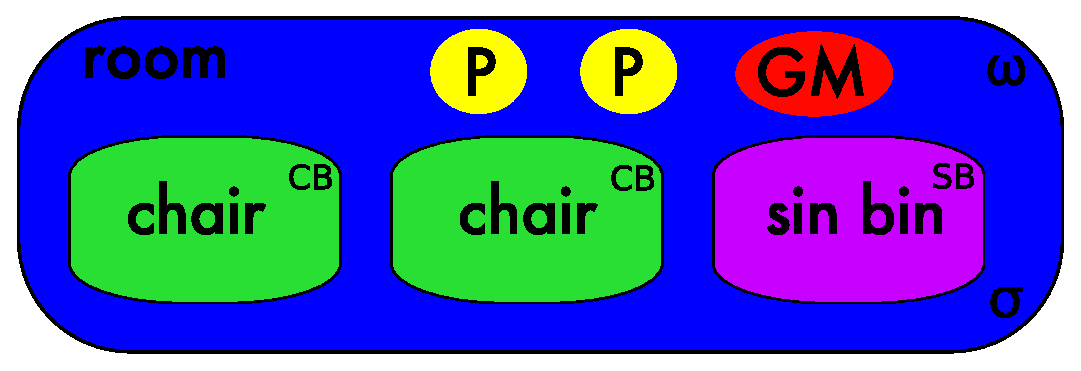
\includegraphics[scale=0.5]{gameenv}
  \caption{The Musical Chairs Environment}
  \label{fig:gameenv}
\end{figure}

The locality structure is represented graphically by Fig. \ref{fig:gameenv}
and in the calculus by the equation shown below.

\begin{equation}
\loc{room}{\nloc{chair}{\nil}{CB} \pc \nloc{chair}{\nil}{CB}
\pc \dots}{\Omega}{\sigma}
\end{equation}

\noindent where $\nloc{m}{E}{F}$ is abbrieviated from
$\loc{m}{E}{F}{\{\}}$.  The players themselves are represented by
\emph{processes}.  This allows them both to interact and to move between
localities.  A gamesmaster process is also introduced.  This doesn't
play an active role in the game itself, but is instead responsible for
performing the administrative duties of removing chairs from the game
and controlling player movement.  The process definitions are summarised
in Table \ref{tab:musicalchairs}, and make use of the derived syntax for
a clock prefix, $\sigma.P$, shown in \ref{clockcontrol}.

\begin{table}[h]
  \caption{Summary of Processes and Derived Syntax for Musical Chairs}
  \label{tab:musicalchairs}
  \shrule
  \begin{align}
   \omega &
     \eqdef 
     \mu X.(\overline{in}.X + \overline{out}.X + \overline{open}.X) \label{o}\\
   \sigma.P &
     \eqdef 
     \stimeout{\nil}{\sigma}{P} \label{clockpref} \\
   CB &
    \eqdef 
    \mu X.(\overline{in}.\overline{out}.X + \overline{open}) \label{chairb} \\
   SB &
    \eqdef 
    \mu X.\overline{in}.X \label{sinb} \\
   GM2 &
    \eqdef 
    \sigma.GM3 \label{gmstage2} \\
    GM3 &
    \eqdef 
    open\ chair.GM5 \label{gmstage3} \\
   GM4 &
   \eqdef
   \sigma.GM4 \label{gmstage4} \\
   GM5 &
    \eqdef  
    \mu X.(\stimeout{in\ chair\ sit.X}{\sigma}{GM6}) \label{gmstage5} \\
   GM6 &
    \eqdef 
    \mu X.(\stimeout{in\ sinbin\ leave.X}{\sigma}{GM2}) \label{gmstage6}\\
    Player &
    \eqdef 
    \stimeout{sit.PInChair}{\sigma}{Loser} \label{player}\\
   PInChair &
    \eqdef 
    \sigma.\sigma.PLeaveChair \label{pinchair} \\
   PLeaveChair &
   \eqdef
   out\ chair\ stand.0|stand.\sigma.\sigma.Player \label{pleavechair} \\
   Loser &
    \eqdef 
    leave.0 \label{loser} 
  \end{align}
  \shrule
\end{table}

The presence of music is signified by the ticks of a clock, $\sigma$.  A
tick from $\sigma$ is also used to represent the implicit
acknowledgement that everyone who can obtain a chair has done so, and
that the remaining player left in the room has lost.  With regard to the
bouncers of the localities, the room locality is not prone to either
destruction or the entry or exit of other localities, having a bouncer
simply equal to $\Omega$.  This retains the encapsulation of the model
as a single room locality, and prevents other processes or localities
from interfering with its behaviour.

The definition of appropriate bouncers is essential for the chairs
(\ref{chairb}) and the sin bin (\ref{sinb}).  It is the chair bouncer
that enforces the implicit predicate that only one player may inhabit a
chair at any one time, while the sin bin bouncer prevents players
leaving the sin bin once they have entered.

To model stage one of the game, $n$ player processes and $n$ chair
locations are placed in the room.  The advantage of using TNT for this
model is that the actual number of players or chairs is irrelevant.
They only have to be equal at the start to accurately model the game.
The calculus allows the creation of a compositional semantics, as
discussed in chapter \ref{introduction}, which work with any $n$.

For the purposes of demonstration, $n$ is assumed to be two to give the
following starting state:

\begin{equation}
  \loc{room}{\nloc{chair}{\nil}{CB} \pc \nloc{chair}{\nil}{CB} \pc 
   \sigma.\sigma.Player \pc \sigma.\sigma.Player \pc GM2}{\Omega}{\sigma}.
\end{equation}

\noindent The room and chairs appear as shown earlier.  The
processes of the form $\sigma.\sigma.Player$ simply wait until two clock
cycles have passed, the end of each being signalled by a tick from
$\sigma$.  The intermittent period between the ticks (the second clock
cycle) represents the playing of the music.  

Stage two, where the music is started, is thus represented simply by the
first tick of $\sigma$,

\begin{equation}
\begin{aligned}
  & \loc{room}{\nloc{chair}{\nil}{CB} \pc \nloc{chair}{\nil}{CB} \pc 
   \sigma.\sigma.Player \pc \sigma.\sigma.Player \pc
   GM2}{\Omega}{\sigma} \\
 \lderives{\sigma}\ & \loc{room}{\nloc{chair}{\nil}{CB} \pc \nloc{chair}{\nil}{CB} \pc 
   \sigma.Player \pc \sigma.Player \pc
   GM3}{\Omega}{\sigma}
\end{aligned}
\end{equation}

\noindent which the gamesmaster ($GM2$ (\ref{gmstage2})) also waits for,
before evolving in to $GM3$ (\ref{gmstage3}).  The second cycle, prior
to the music stopping, is used to remove a chair from the game.  Maximal
progress, as explained in section \ref{introduction}, ensures that this
occurs before the next clock tick, as the removal emits a silent action.
The transition from stage three to stage four is thus as follows:

\begin{equation}
\begin{aligned}
& \loc{room}{\nloc{chair}{\nil}{CB} \pc \nloc{chair}{\nil}{CB} \pc 
   \sigma.Player \pc \sigma.Player \pc
   GM3}{\Omega}{\sigma} \\
 \lderives{\tau}\ & \loc{room}{\nil \pc \nloc{chair}{\nil}{CB} \pc 
   \sigma.Player \pc \sigma.Player \pc
   GM4}{\Omega}{\sigma}
\end{aligned}
\end{equation}

\noindent with one of the two chairs being chosen non-deterministically.
The second tick then occurs, leading in to stage five and the most
interesting part of the model.

\begin{equation}
\begin{aligned}
& \loc{room}{\nil \pc \nloc{chair}{\nil}{CB} \pc 
   \sigma.Player \pc \sigma.Player \pc
   GM4}{\Omega}{\sigma} \\
\lderives{\sigma}\ & \loc{room}{\nil \pc \nloc{chair}{\nil}{CB} \pc 
   Player \pc Player \pc
   GM5}{\Omega}{\sigma} \\
\end{aligned}
\end{equation}

The aim of stage five is to get as many player processes as possible
inside chair localities.  This is handled by again relying on maximal
progress to essentially perform a form of broadcast that centres on
mobile actions, as briefly mentioned in \ref{procmob}.  Rather than
sending a signal to a number of recipients, a request to move into a
chair (see (\ref{gmstage5}) and (\ref{player})) is delivered instead.

If a chair is available, then a player process will enter it (the actual
chair and player chosen is non-deterministic).  This will cause an
internal action to occur, which takes precedence over the clock tick.
Thus, when the clock eventually does tick, it is clear that no more
players can enter chairs. Using clocks in this manner makes the system
\emph{compositional}; in contrast to other models, players and chairs
can be added without requiring changes to the process definitions.  In
this running example, there are two players, but only one chair, which
results in a single $\tau$ transition:

\begin{equation}
\begin{aligned}
& \loc{room}{\nil \pc \nloc{chair}{\nil}{CB} \pc 
   Player \pc Player \pc
   GM5}{\Omega}{\sigma} \\
\lderives{\tau}\ & \loc{room}{\nil \pc \nloc{chair}{\nil \pc PInChair}{\overline{out}.CB} \pc 
   Player \pc
   GM5}{\Omega}{\sigma} \\
\end{aligned}
\end{equation}

\noindent that causes one of the $Player$ processes to move in to a
chair, and become a $PInChair$ process.  This is followed by the
$\sigma$ transition, which marks the move to stage six.

\begin{equation}
\begin{aligned}
&  \loc{room}{\nil \pc \nloc{chair}{\nil \pc PInChair}{\overline{out}.CB} \pc 
   Player \pc
   GM5}{\Omega}{\sigma} \\
\lderives{\sigma}\ & \loc{room}{\nil \pc \nloc{chair}{\nil \pc \sigma.PLeaveChair}{\overline{out}.CB} \pc 
   Loser \pc
   GM6}{\Omega}{\sigma} \\
\end{aligned}
\end{equation}

Both stage six and seven proceed in a similar way.  Stage six sees
essentially the same broadcasting behaviour applied to the losing
players (see (\ref{gmstage6}) and (\ref{loser})).  The difference is
that stage six demonstrates something which wouldn't be possible without
mobility: the broadcast is limited to those player processes which
remain in the room.  As communication between processes in different
localities is disallowed in TNT, an implicit scoping of the broadcast
occurs.  In the example, stage six again sees just one $\tau$
transition:

\begin{equation}
\begin{aligned}
&  \loc{room}{\nil \pc \nloc{chair}{\nil \pc \sigma.PLeaveChair}{\overline{out}.CB} \pc 
   Loser \pc
   GM6}{\Omega}{\sigma} \\
\lderives{\tau}\ & \loc{room}{\nil \pc \nloc{chair}{\nil \pc \sigma.PLeaveChair}{\overline{out}.CB} \pc
   GM6}{\Omega}{\sigma} \\
\end{aligned}
\end{equation}

\noindent which results in the remaining $Player$ (now a $Loser$
process) moving to the sin bin.  Due to space constraints, the sin bin
locality is not shown in the above derivations.  It may be factored in
to the above as follows:

\begin{equation}
\begin{aligned}
& \nloc{sinbin}{\nil}{SB} \pc Loser \pc GM6 \\
\lderives{\tau} & \nloc{sinbin}{\nil \pc \nil}{SB} \pc GM6
\end{aligned}
\end{equation}

\noindent where the $Loser$ process evolves to become a simple $\nil$
process.  The broadcast is again terminated by a tick from $\sigma$,

\begin{equation}
\begin{aligned}
&  \loc{room}{\nil \pc \nloc{chair}{\nil \pc \sigma.PLeaveChair}{\overline{out}.CB} \pc
   GM6}{\Omega}{\sigma} \\
\lderives{\sigma}\ & \loc{room}{\nil \pc \nloc{chair}{\nil \pc PLeaveChair}{\overline{out}.CB} \pc
   GM2}{\Omega}{\sigma} 
\end{aligned}
\end{equation}

\noindent which, in this case, also signifies the music starting up again.  The
remaining players leave their chairs:

\begin{equation}
\begin{aligned}
& \loc{room}{\nil \pc \nloc{chair}{\nil \pc PLeaveChair}{\overline{out}.CB} \pc
   GM2}{\Omega}{\sigma}   \\
\lderives{\tau}\ & \loc{room}{\nil \pc \nloc{chair}{\nil \pc \nil}{CB} \pc
   GM2 \pc \sigma.\sigma.Player}{\Omega}{\sigma} 
\end{aligned}
\end{equation}

\noindent and the system essentially returns to the beginning, with $n -
1$ chairs and $n - 1$ players.

\section{The Type System}
\label{typesys}

This final section focuses on the beginnings of a type system for the
calculus.  The concepts behind this are based on the type systems
presented for the ambient calculus (see \ref{ambienttypes}) and
specifically the notion of groups presented in \cite{ambienttypes} and
\cite{m3}.  The current focus is on further restricting mobility, this
time limiting which process may move rather than how many, as is implied
by the bouncers of \ref{bouncers}.  The type system also provides the
distinction between normal process primitives and the primitives used by
bouncers, which is implicit in the examples above.

Each process and locality is a member of a group, which determines the
use of the mobility primitives.  Each group has a type\footnote{Or, as
groups are types themselves, it essentially has a type of a type or a
\emph{kind}}, $(\mathscr{C}, \mathscr{S}, \mathscr{O})$, with each
element being a set of groups.  Entities in groups that are members of
$\mathscr{C}$ are allowed to cross or pass through localities in the
given group.  For example, if $g_1$ has type $G_1$, where
$\mathscr{C}(G_1)$ is ${g_2}$, then localities or processes in group
$g_2$ may cross through localities in $g_1$.  In the same way,
$\mathscr{S}$ is the set of groups that may stay in a locality of that
group.  This is implicity a subset of $\mathscr{C}$ as, if a locality
can be stayed in, it must be crossable too.  Finally, $\mathscr{O}$
controls the members of which groups may destroy the locality via the
$open$ primitive.

Table \ref{tab:basictypes} presents the basic rules and the rudimentary
types used for the basic parts of the syntax, such as $\nil$.  As is
standard in the literature, the types are defined with respect to a type
environment, $\Gamma$.  On this note, the rule $Env$ simply states that
if $\xi$ of type $T$ is a member of $\Gamma$, then a typing derivation
$\vdash \xi : T$ may be made in the context of $\Gamma$.  This forms the
basis of all later rules.

\begin{table}
  \caption{Types: Basics}
  \label{tab:basictypes}
  \shrule
 \begin{center}
 \begin{tabular}{rc}
     \Rule{Env}
     {\xi : T \in \Gamma}
     {\Gamma \vdash \xi : T}
     {}
  &
  \Rule{Nil}
     {-}
     {\Gamma \vdash \nil : Proc(g)}
     {}
  \\[3ex]
     \Rule{BNil}
     {-}
     {\Gamma \vdash \Omega : BProc}
     {}
     &
     \Rule{Stop}
     {-}
     {\Gamma \vdash \Delta : Proc(g)}
     {}
     \\[3ex]
     \Rule{Stall}
     {\Gamma \vdash \sigma : Clock}
     {\Gamma \vdash \Delta_\sigma : Proc(g)}
     {}
     &
     \Rule{Act}
     {\Gamma \vdash \alpha : Act,
     \Gamma \vdash P : Proc (g)}
     {\Gamma \vdash \alpha . P : Proc(g)}
     {}
  \\[3ex]
     \Rule{Rec}
     {\Gamma \vdash P : Proc(g)}
     {\Gamma \vdash \mu X.P : Proc(g)}
     {}
     &
     \Rule{Res}
     {\Gamma \vdash a : Act,
     \Gamma \vdash P : Proc (g)}
     {\Gamma \vdash P \setminus a : Proc(g)}
     {}
 \end{tabular}
  \end{center}
  \shrule
\end{table}

The remaining rules in Table \ref{tab:basictypes} provide types for the
processes.  Via $Nil$ and $Stop$, both $\nil$ and $\Delta$ are given a
type of $Proc(g)$, where $g$ is a group.  There are no preconditions for
these derivations.  Likewise, $\Omega$ can be typed as a $BProc$, a
bouncer process, thus distinguishing it from the normal processes, such
as $\nil$.

The other rules are also pretty simple.  $Stall$ simply says that
$Delta_{\sigma}$ may be typed as a process of group $g$ if $\sigma$ is a
clock.  $Act$ states that $\alpha.P$ is a process in $g$ if $\alpha$ is
an action and $P$ is also typeable as a process in the same group.  In
the same vein, $Rec$ and $Res$ type recursive and restricted processes
respectively, if the constituent process, $P$, is already typeable as a
process.  In the case of $Res$, $a$ must also be an action if the
process is to be successfully typed.

In Table \ref{tab:operatortypes}, types are given to the composition of
processes using the binary operators for summation, parallel composition
and timeout.  All four are pretty much identical, providing a type for
the process resulting from the combination of the operator with two
other processes, $P$ and $Q$.  As each of these processes may be typed
under a different type environment (represented by $\Gamma_1$ and
$Gamma_2$), the cumulative process is typed under the union of the two,
on the condition that the two are compatible ($\Gamma_1 \# \Gamma_2$).
Compatibility is possible if there is no overlap between the two
environments.  Such overlap occurs when both environments provide a
different type for the same entity.  

\begin{table}
  \caption{Types: Operators}
  \label{tab:operatortypes}
  \shrule
 \begin{center}
 \begin{tabular}{c}
     \Rule{Sum}
     {\Gamma_1 \vdash P : Proc(g),
      \Gamma_2 \vdash Q : Proc(g),
      \Gamma_1 \# \Gamma_2}
     {\Gamma_1 \cup \Gamma_2 \vdash P + Q : Proc(g)}
     {}
     \\[3ex]
     \Rule{Par}
     {\Gamma_1 \vdash P : Proc(g),
      \Gamma_2 \vdash Q : Proc(g),
      \Gamma_1 \# \Gamma_2}
     {\Gamma_1 \cup \Gamma_2 \vdash P \;|\; Q : Proc(g)}
     {}
     \\[3ex]
     \Rule{FTO}
     {\Gamma_1 \vdash P : Proc(g),
      \Gamma_2 \vdash Q : Proc(g),
      \Gamma_1 \# \Gamma_2,
      \Gamma_1 \cup \Gamma_2 \vdash \sigma : Clock}
     {\Gamma_1 \cup \Gamma_2 \vdash \timeout{P}{\sigma}{Q} : Proc(g)}
     {}
  \\[3ex]
  \Rule{STO}
  {\Gamma_1 \vdash P : Proc(g),
      \Gamma_2 \vdash Q : Proc(g),
      \Gamma_1 \# \Gamma_2,
      \Gamma_1 \cup \Gamma_2 \vdash \sigma : Clock}
     {\Gamma_1 \cup \Gamma_2 \vdash \stimeout{P}{\sigma}{Q} : Proc(g)}
     {}
     \\[3ex]
 \end{tabular}
  \end{center}
  \shrule
\end{table}

The only other issue worthy of note with respect to these rules is that
$FTO$ and $STO$ also require that $\sigma$ is typeable as a clock,
another restriction which simply makes explicit a number of issues
implied in the syntax.

The types in Tables \ref{tab:basictypes} and \ref{tab:operatortypes}
provide the basis for the mobility types presented in Table
\ref{tab:mobilitytypes}, which form the focus of the type system.  This
table is so far incomplete, as it lacks typing for process mobility and
the rule to link processes and localities.  The latter exists, but may
need further work.  These issues are discussed in \ref{futuretypes}.

\begin{table}
  \caption{Types: Mobility}
  \label{tab:mobilitytypes}
  \shrule
 \begin{center}
 \begin{tabular}{c}
     \Rule{Cap}
     {\Gamma \vdash \ambop : Proc(g_1) \rightarrow Proc(g_2),
     \Gamma \vdash P : Proc (g_1)}
     {\Gamma \vdash \ambop . P : Proc(g_2)}
     {}
     \\[3ex]
     \Rule{LocIn}
     {\Gamma \vdash g_2 : G_2,
      \Gamma \vdash m : Loc(g_1),
      g_1 \in \mathscr{C}(G_2)}
     {\Gamma \vdash \ambin{m} : Proc(g_2) \rightarrow Proc(g_2)}
     {}
     \\[3ex]
     \Rule{LocOut\ }
     {\Gamma \vdash g_1 : G_1, 
      \Gamma \vdash g_2 : G_2,
      \Gamma \vdash m : Loc(g_1),
      g_1 \in \mathscr{C}(G_2),
      \mathscr{S}(G_1) \subseteq \mathscr{S}(G_2)}
     {\Gamma \vdash \ambout{m} : Proc(g_2) \rightarrow Proc(g_2)}
     {}
     \\[3ex]
     \Rule{Open}
     {\Gamma \vdash g_1 : G_1,
      \Gamma \vdash g_2 : G_2,
      \Gamma \vdash m : Loc(g_1),
      g_1 \in \mathscr{O}(G_2),
      g_2 \in \mathscr{S}(G_1)}
     {\Gamma \vdash \ambopen{m} : Proc(g_2) \rightarrow Proc(g_2)}
     {}
 \end{tabular}
  \end{center}
  \shrule
\end{table}

Of the ones presented here, $LocIn$, $LocOut$ and $Open$ are fairly
similar, all relating to whether a particular location movement is
typeable, based on the groups of the localities and the processes within
them.  $Cap$ differs in that it provides the actual change in type that
occurs when the movement takes place.  Its behaviour is akin to function
composition.  

Within the type system, mobility primitives are given function types, to
represent the fact that they may cause a transition from one group to
another\footnote{This is not evident in the rules given, as the
processes move as part of the locality, and thus stay in the same
group.  Such changes occur in process movement, where the locality of a
process changes, and thus its group.}.  The rule itself simply states
that if $\ambop$ has a function type, transforming processes of the
group $g_1$ to a process in the group $g_2$, and $P$ is a process in
group $g_1$, then $\ambop.P$ is typed as the result of applying $\ambop$
to $P$, to give a process in group $g_2$.

The function types used for this are generated by rules like $LocIn$,
$LocOut$ and $Open$, which are specific to each mobility primitive.
$LocIn$ states that if $m$ is a locality of group $g_1$, then
$\ambin{m}$ is typeable as $Proc(g_2) \rightarrow Proc(g_2)$ if the
group $g_1$ is one of the members of the set of crossable localities
maintained by $G_2$, the type of the group, $g_2$, used by the process
emitting the capability.

The other two rules run along the same lines.  $LocOut$ is nearly the
same, except that the set of locality groups where members of $g_1$ can
stay must be a subset of the set in which members of $g_2$ can stay.
This is because the moving locality, in $g_1$, must be able to stay in
the locality in which $m$ (a member of $g_2$) is currently situated,
when it moves outside it.

Finally, the rule for $Open$ states that $g_1$, the group of the
locality being opened, must be a member of the set of groups that are
openable by members of $g_2$ and that $g_2$ must be a member of the set
of groups that can stay in localities of group $g_1$.  The latter
condition is necessary to ensure that the contents of the destroyed
locality are allowed to enter the parent locality.

